\documentclass[final]{beamer}\usepackage[]{graphicx}\usepackage[]{color}
%% maxwidth is the original width if it is less than linewidth
%% otherwise use linewidth (to make sure the graphics do not exceed the margin)
\makeatletter
\def\maxwidth{ %
  \ifdim\Gin@nat@width>\linewidth
    \linewidth
  \else
    \Gin@nat@width
  \fi
}
\makeatother

\definecolor{fgcolor}{rgb}{0.345, 0.345, 0.345}
\newcommand{\hlnum}[1]{\textcolor[rgb]{0.686,0.059,0.569}{#1}}%
\newcommand{\hlstr}[1]{\textcolor[rgb]{0.192,0.494,0.8}{#1}}%
\newcommand{\hlcom}[1]{\textcolor[rgb]{0.678,0.584,0.686}{\textit{#1}}}%
\newcommand{\hlopt}[1]{\textcolor[rgb]{0,0,0}{#1}}%
\newcommand{\hlstd}[1]{\textcolor[rgb]{0.345,0.345,0.345}{#1}}%
\newcommand{\hlkwa}[1]{\textcolor[rgb]{0.161,0.373,0.58}{\textbf{#1}}}%
\newcommand{\hlkwb}[1]{\textcolor[rgb]{0.69,0.353,0.396}{#1}}%
\newcommand{\hlkwc}[1]{\textcolor[rgb]{0.333,0.667,0.333}{#1}}%
\newcommand{\hlkwd}[1]{\textcolor[rgb]{0.737,0.353,0.396}{\textbf{#1}}}%
\let\hlipl\hlkwb

\usepackage{framed}
\makeatletter
\newenvironment{kframe}{%
 \def\at@end@of@kframe{}%
 \ifinner\ifhmode%
  \def\at@end@of@kframe{\end{minipage}}%
  \begin{minipage}{\columnwidth}%
 \fi\fi%
 \def\FrameCommand##1{\hskip\@totalleftmargin \hskip-\fboxsep
 \colorbox{shadecolor}{##1}\hskip-\fboxsep
     % There is no \\@totalrightmargin, so:
     \hskip-\linewidth \hskip-\@totalleftmargin \hskip\columnwidth}%
 \MakeFramed {\advance\hsize-\width
   \@totalleftmargin\z@ \linewidth\hsize
   \@setminipage}}%
 {\par\unskip\endMakeFramed%
 \at@end@of@kframe}
\makeatother

\definecolor{shadecolor}{rgb}{.97, .97, .97}
\definecolor{messagecolor}{rgb}{0, 0, 0}
\definecolor{warningcolor}{rgb}{1, 0, 1}
\definecolor{errorcolor}{rgb}{1, 0, 0}
\newenvironment{knitrout}{}{} % an empty environment to be redefined in TeX

\usepackage{alltt}
\usefonttheme{serif}
\mode<presentation>{\usetheme{ASU}}
\usepackage{amsmath, amsfonts, amssymb, pxfonts, eulervm, xspace, enumerate, hyperref, color, bookmark}
\usepackage{graphicx}
\usepackage[orientation=landscape, size=a0, scale=1.4, debug]{beamerposter}
% \usepackage{natbib}

\usecolortheme{rose}
\setbeamercolor{background canvas}{bg=white!16!white!90}


%-- Header and footer information ----------------------------------
\newcommand{\footright}{\href{https://github.com/STAT-ATA-ASU/STT3851Spring2016}{https://github.com/STAT-ATA-ASU/Padgett-Averia/tree/master/Assignments2017/KingsCounty}}
\newcommand{\footleft}{\href{mailto:arnholtat@appstate.edu}{Faculty Advisor: Alan Arnholt}}

\def\conference{King County House Price Prediction Project}
\title{Price Prediction Project}
\author{Cescily Metzgar, Averia Padgett} 
\institute{Department of Mathematical Sciences}
%-------------------------------------------------------------------


%-- Main Document --------------------------------------------------
\IfFileExists{upquote.sty}{\usepackage{upquote}}{}
\begin{document}
\begin{frame}[fragile]
\vspace{-2ex}
\begin{columns}[t]



%-- Column 1 ---------------------------------------------------
\begin{column}{0.31\linewidth}
\begin{minipage}[t][.955\textheight]{\linewidth} 

%-- Block 1-1
\vspace{0ex}
\begin{block}{Overview}
\begin{itemize}
\item This poster examines housing data from King's County and aims to predict prices of houses based on different variables.  
\item To ensure accurate predictive power for future observations, the data are split into a training set (80\%) and a test set (20\%). 
\item Root mean squared error of the test set is used as a measure of model adequacy.  
\item All computations and graphs are created with the open source software \texttt{R} \cite{R-base}. 
\end{itemize}
\vspace{0ex}
\end{block}
\vfill

%-- Block 1-2
\begin{block}{Residual Plots}
\begin{itemize}
\item A residual plot is a graph that shows the residuals on the vertical axis and the independent variable on the horizontal axis. If the points in a residual plot are randomly dispersed around the horizontal axis, a linear regression model is appropriate for the data; otherwise, a non-linear model is more appropriate.
\vspace{2ex}
\item Using the residual plots we found variables that need to be made non-linear to create a more randomly distributed residual plot so that the variables can be used in a linear model. 

\begin{knitrout}
\definecolor{shadecolor}{rgb}{0.969, 0.969, 0.969}\color{fgcolor}

{\centering \includegraphics[width=\maxwidth]{figure/unnamed-chunk-1-1} 

}




{\centering 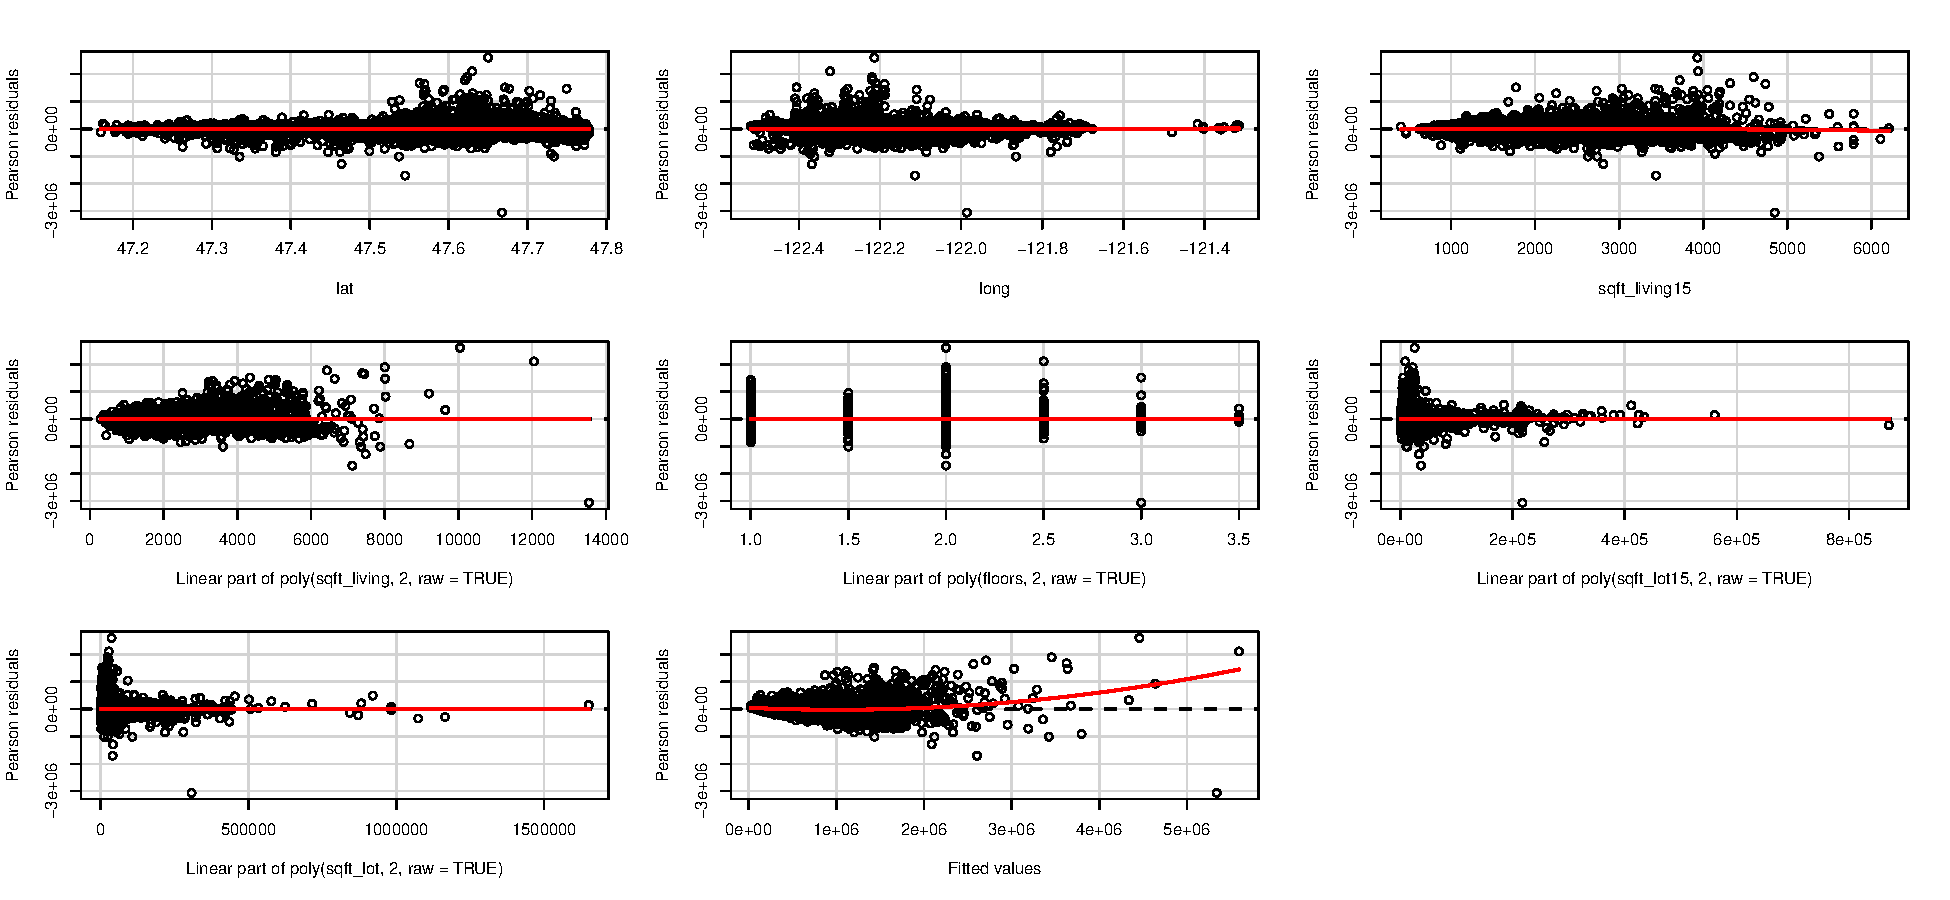
\includegraphics[width=\maxwidth]{figure/unnamed-chunk-1-2} 

}



\end{knitrout}
\vspace{2ex}
\item In the above residual plots the variables sqft\_living, floors, sqft\_lot15, and sqft\_lot were squared which resulted in an almost perfectly distributed residuals for each variable. 
\end{itemize}
\vspace{0ex}
\vfill
\end{block}
\vfill

\end{minipage}
\end{column}%1

%-- Column 2 ---------------------------------------------------

\begin{column}{0.31\linewidth}
\begin{minipage}[t][.955\textheight]{\linewidth} 

%-- Block 2-1
\vspace{0ex}
\begin{block}{Basic Models Used}
\begin{itemize}
\item Backwards Elimination: The backwards elimination approach takes mod2 as the full model and works backwards to eliminate variables until it produces the best model, resulting in the lowest AIC possible.  
\item Forward Selection: The forward selection approach takes a null model, a model that is basically empty, and adds variables individually until the best model is produced, resulting in the lowest AIC possible.   
\item Interaction Model: Examines the interactions between various variables.
\end{itemize}
\vspace{0ex}
\end{block}
\vfill

%-- Block 2-2
\vspace{0ex}
\begin{block}{King County Real Estate}
\vspace{0ex}
\begin{knitrout}
\definecolor{shadecolor}{rgb}{0.969, 0.969, 0.969}\color{fgcolor}\begin{kframe}


{\ttfamily\noindent\bfseries\color{errorcolor}{Error in get("{}f"{}, environment(CoordMap\$train)): object 'f' not found}}\end{kframe}
\end{knitrout}
\vspace{0ex}
\end{block}
\vfill

\end{minipage}
\end{column}%2

%-- Column 3 ---------------------------------------------------
\begin{column}{0.31\linewidth}
\begin{minipage}[t][.955\textheight]{\linewidth} 

%-- Block 3-1
\vspace{0ex}
\begin{block}{Backwards Elimination}
\begin{itemize}
\item Below is the model backwards elimination produced. After running a summary of the model it produced an Adjusted R-squared value of  0.8416. 
\vspace{1ex}
\begin{center}\includegraphics[width=12in]{picture1.png}\end{center}
\end{itemize}
\vspace{0ex}
\end{block}
\vfill

%-- Block 3-2
\vspace{0ex}
\begin{block}{Forward Selection}
\begin{itemize}
\item Below is the model forward selection produced. After running a summary of the model it produced an Adjusted R-squared value of  0.8416, the same Adjusted-R squared backwards elimination produced. \vspace{1ex}
\begin{center}\includegraphics[width=12in]{picture2.png}\end{center}
\end{itemize}
\vspace{0ex}
\end{block}
\vfill

%-- Block 3-3
\vspace{0ex}
\begin{block}{Interaction Model}
\begin{itemize}
\item Below  is the interaction model created to predict house price using various interaction terms. The following interaction terms were included in this model: bedrooms:bathrooms, sqft\_living15:sqft\_living, condition:grade, yr\_built:yr\_renovated, and zipcode:long. This model resulted in an Adjusted-R squared value of 0.8606 which is higher than both backwards elimination and forward selection. 
\vspace{1ex}
\begin{center}\includegraphics[width=12in]{picture3.png}\end{center}
\end{itemize}
\vspace{0ex}
\end{block}
\vfill

%-- Block 3-4
\begin{block}{References}
\footnotesize
\setbeamertemplate{bibliography item}[text]
\vspace{-1ex}


\bibliographystyle{plain}  % can use plain but comment out natbib at top if using plain
\bibliography{knitr-packages,poster}
\normalsize
\vfill
\end{block} 
\vfill

\end{minipage}
\end{column}%3




\end{columns}
\end{frame}
\end{document}

